 
\section{系统设计}
\label{sec:sys}

\begin{figure}[!t]
  \centering
  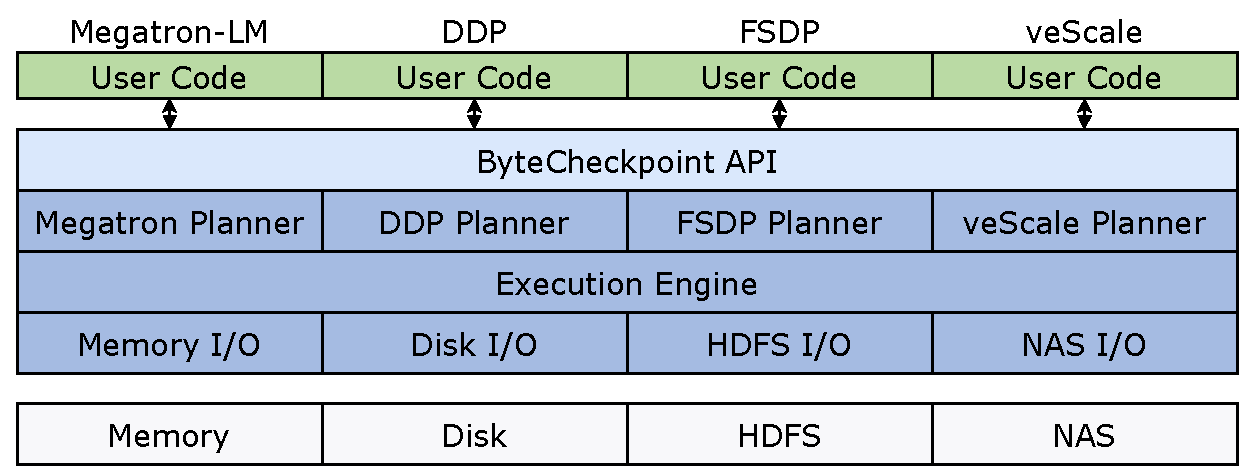
\includegraphics[width=\linewidth]{figures/architecture.pdf}
  \caption{\sys{} 的架构。
  }
  \label{fig:architecture}
\end{figure}

基于上述观察，我们按照以下关键原则设计 \sys{}：

\noindent \textit{(1) 解耦}。
checkpoint 表示与具体运行时 parallelism 保持独立。
训练框架与 storage backend 的接口与核心执行引擎分离，确保良好的可扩展性。

\noindent \textit{(2) 易用性}。
API 应当简洁，便于 AI 研究人员与工程师无缝集成到代码与运行环境中。

\subsection{统一架构}
\label{sec:arch}
\sys{} 的架构如图~\ref{fig:architecture} 所示。各组件如下：

\noindent \textbf{API。} \sys{} 的 API（\texttt{bytecheckpoint.save} 与 \texttt{bytecheckpoint.load}）为不同训练框架的用户提供统一入口。
例如保存 checkpoint 时，用户准备好训练状态、checkpoint 路径、框架名称与性能相关选项，然后调用 \texttt{bytecheckpoint.save}。
该高层入口屏蔽了底层复杂度，例如分片规范、保存/reshard plan 生成与 I/O 操作。

\noindent \textbf{Planner。}
Planner 是训练框架的接口层。
它从 API 层接收参数（训练状态、checkpoint 路径等），根据 worker 的 rank 与框架特定的分片规范（如 \textit{Megatron ShardedTensor} 或 \textit{FSDP DTensor}）为每个 tensor shard 创建 ShardMeta（Sec.~\ref{sec:represent}），并决定每个 worker 需要保存/加载的 tensor 与其他状态。
每个 worker 先生成本地 plan，再协同生成全局 plan。
我们为每个训练框架实现定制化 planner，以抽取这些规范信息并生成 plans。

\noindent \textbf{Execution Engine。}
引擎运行在每个训练 worker 上，当调用相应 API 时执行 Planner 生成的保存/加载 plans。
它解析 checkpoint 路径以确定对应的 storage backend，并与 Storage I/O 层交互以执行 plans 中的 I/O 任务。

\noindent \textbf{Storage I/O。}
与 Planner 层类似，Storage I/O 层封装不同 storage backend，并管理后端特定的读写操作与优化。
Engine 与 Storage I/O 层之间保持统一接口，便于无缝集成新的 storage backend。
\sys{} 支持多种 storage 选项，包括 in-memory checkpoint 存储~\cite{gemini-sys}、本地磁盘存储与远程存储系统。

\begin{figure}[!t]
  \centering
  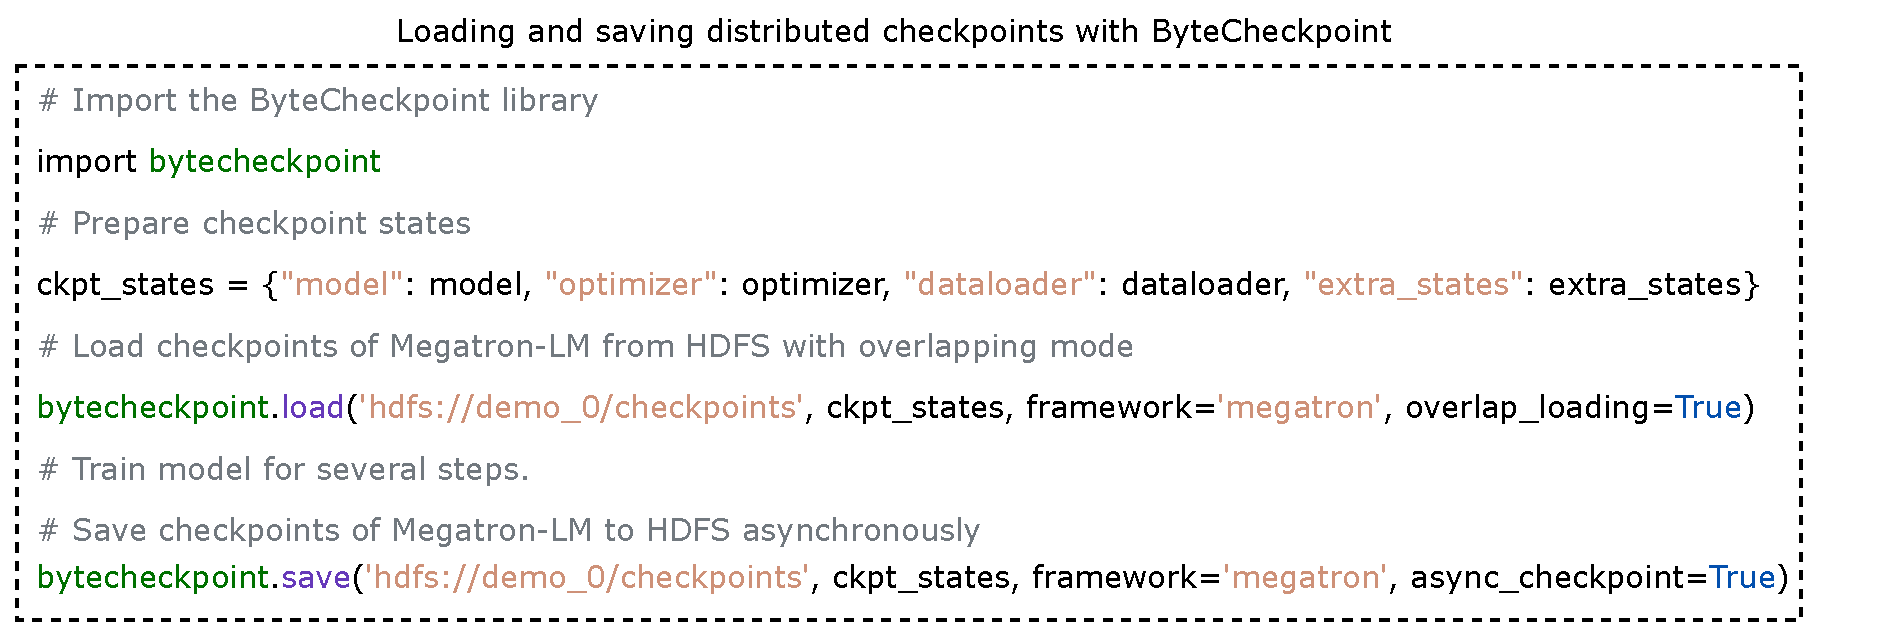
\includegraphics[width=\linewidth]{figures/code_examples.pdf}
  \caption{\sys{} API 的使用示例。
  }
  \label{fig:code_examples}
\end{figure}

图~\ref{fig:code_examples} 展示了 \sys{} 的典型使用方式。
首先，用户定义一个字典，指定需要保存或加载的状态（模型、优化器、dataloader 以及其他状态）。
在训练恢复、阶段切换或 evaluation 开始时调用 \texttt{bytecheckpoint.load} 以加载已保存的 checkpoints。
当 parallelism 发生变化时，checkpoint resharding 会在加载过程中自动完成。
训练过程中，\texttt{bytecheckpoint.save} 会周期性调用以保存 checkpoints。

\subsection{解耦的 Checkpoint 表示}\label{sec:represent}
% Give an overview here.
% How a checkpoint can be represented.

%\noindent \textbf{Sharding spec.}
为了实现与 parallelism 无关的 checkpointing 并支持自动 load-time resharding，我们提出分布式训练中模型与优化器张量的形式化表示规范。
该设计与 \textit{PyTorch Distributed} 库~\cite{ddp} 中的 Distributed Tensor 与 Checkpoint 概念保持一致。

\noindent \textbf{模型与优化器状态。}
每个 tensor 由唯一的“fully qualified name”（FQN）标识，并具有全局形状，表示分片前的原始形状。
Tensor 可以在不同 rank（训练 worker）间分片或复制。
对于分片 tensor，每个 worker 持有的 shard 由三类信息决定：该 tensor 所采用的 parallelism（如 tensor parallelism）、分片维度、以及在对应 parallelism group 内的 group rank。
基于 tensor 的 FQN、全局形状与分片规范，\sys{} 为每个 rank 创建 tensor shard 的 metadata（ShardMeta），用于在 checkpoint 中表示该 shard，且与具体 parallelism 无关。
具体而言，ShardMeta 是一个索引元组 \textit{(fqn, nD\_offsets, nD\_lengths)}，其中 \textit{nD\_offsets} 与 \textit{nD\_lengths} 表示该 shard 在原始多维形状上的偏移与长度。

\begin{figure}[!t]
  \centering
  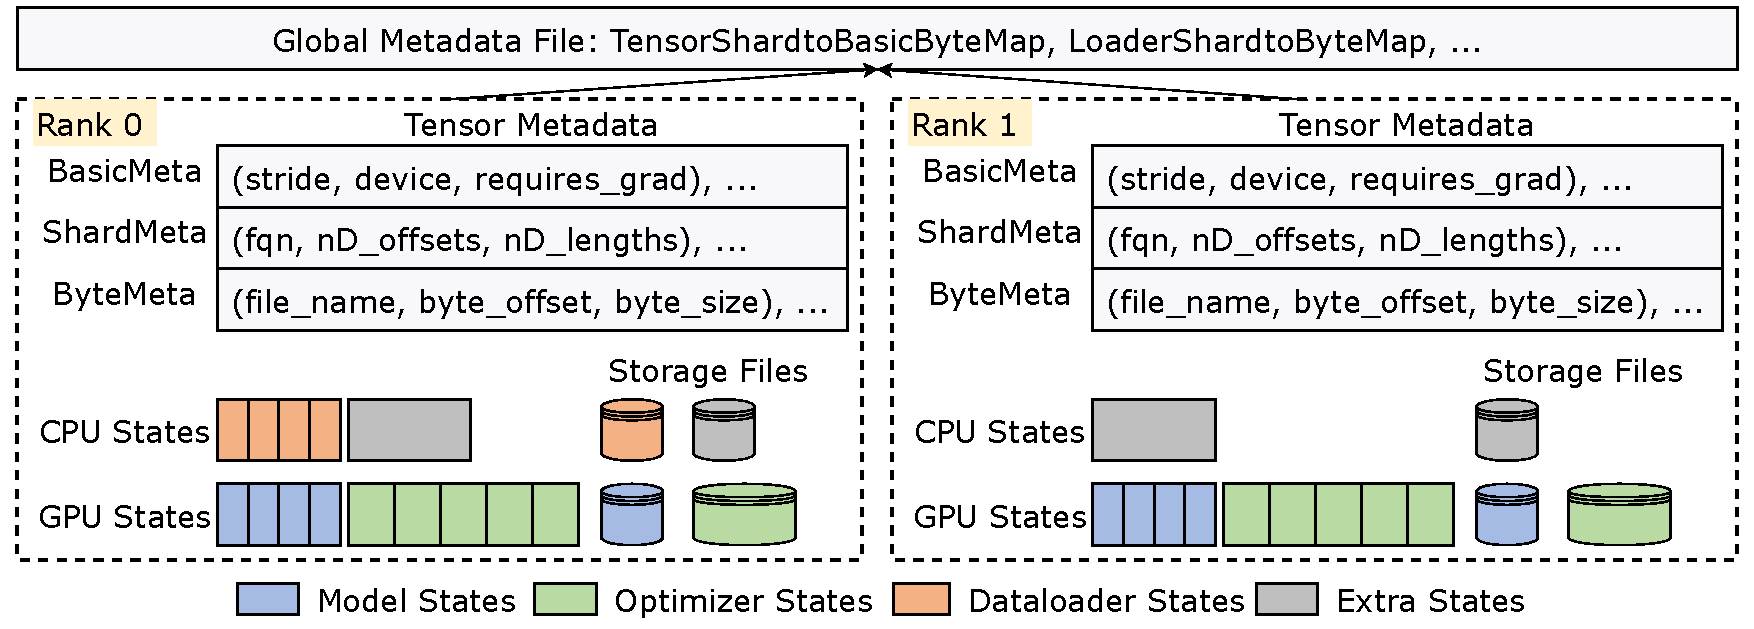
\includegraphics[width=\linewidth]{figures/representation.pdf}
  \caption{
  \sys{} 中的 checkpoint 表示。
  该示例采用 pipeline parallelism。
  }
  \vspace{-5mm}
  \label{fig:representation_meta}
\end{figure}

\noindent \textbf{Dataloader 与其他状态。}
Dataloader 状态可划分为两类：\textit{replicated} 状态与 \textit{sharded} 状态。
replicated 状态包含数据读取 worker 数、数据源路径与采样比例等信息，且在不同 rank 的所有 I/O worker（子进程）之间一致。
sharded 状态在每个 I/O worker 间不同，包括 token buffer 与各数据源的读取偏移。
在 \sys{} 中，sharded 状态保存为独立文件，而 replicated 状态仅由 rank 0 的 I/O worker 保存。
该策略减少了需保存的 dataloader 状态总体大小，并在 parallelism 变化时便于 dataloader resharding，因为将数据状态拆分为独立文件能简化合并与重分配过程。
对于 RNG 等其他额外状态，我们将其打包并序列化为一个紧凑的字节对象后写入存储。

\noindent \textbf{Checkpoint 表示。}
图~\ref{fig:representation_meta} 展示了 \sys{} 的 checkpoint 表示。
分布式 checkpoints 由一个 \textit{全局 metadata 文件} 与多个 \textit{存储文件} 组成。
每个 rank 生成三类文件：模型状态文件、优化器状态文件与额外状态文件。
dataloader 状态文件仅由除 DP 之外各 parallelism 度的 rank 为 0 的训练 worker 生成。
对于模型与优化器状态中的 tensor shards，其 \textit{metadata} 由三部分组成：
\textit{BasicMeta}（记录单个 tensor shard 的必要信息，如 stride 与 device，用于恢复运行时状态）；
\textit{ShardMeta}（记录 shard 在完整 tensor 中的位置）；
\textit{ByteMeta}（记录该 shard 在存储文件中的字节起始偏移与长度）。
所有 tensor metadata 被汇总到全局 metadata 文件中，并基于每个 shard 的 ShardMeta、BasicMeta 与 ByteMeta 建立映射 \textit{TensorShardtoBasicByteMap}，确保准确取回数据。
全局 metadata 文件还包含 \textit{LoaderShardtoByteMap}，记录每个 dataloader 中 sharded 状态的文件索引信息。
所有存储文件与全局 metadata 文件都保存在 checkpoint 路径指定的 storage backend 中。

\begin{figure}[!t]
  \centering
  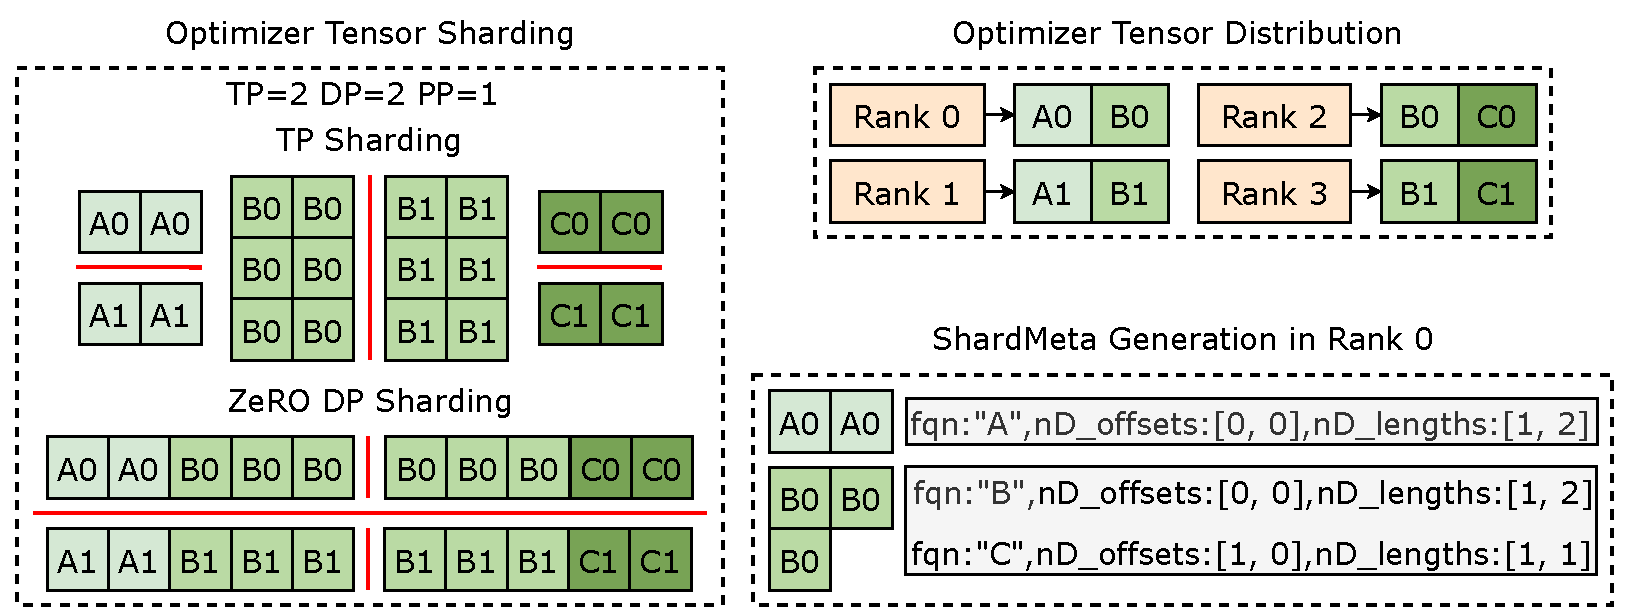
\includegraphics[width=\linewidth]{figures/irregular_tensor.pdf}
  \caption{
  优化器状态中 irregular tensor 的 ShardMeta。
  }
  \label{fig:irregular_decomposed_meta}
  \vspace{-5mm}
\end{figure}

\noindent \textbf{Irregular tensor 分解。}
我们将 irregular tensor 定义为：在分片前被扁平化后，无法恢复回原始维度的 tensor。
这类 tensor 通常出现在 Zero Redundancy Optimizer（ZeRO）~\cite{zero} 的实现中，例如 Megatron-LM ZeRO2 与 FSDP ZeRO3~\cite{fsdp}。
在这些实现中，DP 组内的优化器状态会被扁平化、拼接并分片，导致得到的 1D tensor 切片无法直接用 n 维形状与偏移描述。
图~\ref{fig:irregular_decomposed_meta} 展示了 irregular tensor 分片示例：与张量 $A$ 和 $C$ 不同，原始形状为 (3, 2) 的张量 $B$ 被均匀分成两个 shard，每个 shard 含 3 个元素，无法直接表示为二维形状及其偏移。
一种直观方案是在保存 checkpoint 前将所有 tensor shards 合并为完整 tensor，以便生成 ShardMeta。
例如，为消除 DCP~\cite{torch-dcp} 中潜在的 irregular tensor，FSDP 会对每个 shard 执行同步 all-gather，并与 D2H 拷贝交错进行，无论该 shard 是否 irregular。
但这种做法带来显著通信开销，并需要频繁 GPU/CPU 同步，严重影响效率。

为降低合并开销，\sys{} 采用 tensor 分解策略处理 irregular tensor shards。
具体来说，\sys{} 将一个 irregular tensor 分解为多个 regular tensor，并用多个索引元组进行表示。
例如，图~\ref{fig:irregular_decomposed_meta} 中 rank 0 上张量 $B$ 的 irregular shard 含 3 个元素，\sys{} 将其分解为两个 regular tensor，可直接由 $nD\_offsets$ 与 $nD\_lengths$ 表示。
因此，\sys{} 使用多个 \textit{ShardMeta} 条目来表示单个 irregular tensor shard。
尽管分解会稍微增大 metadata 体积并增加加载过程（重建目标 tensor 可能需要查找多个小片段），但它避免了保存阶段昂贵的 shard 通信，同时不引入额外阻塞。

\subsection{Checkpoint Resharding 工作流}
\label{sec:workflow}

\begin{figure}[!t]
  \centering
  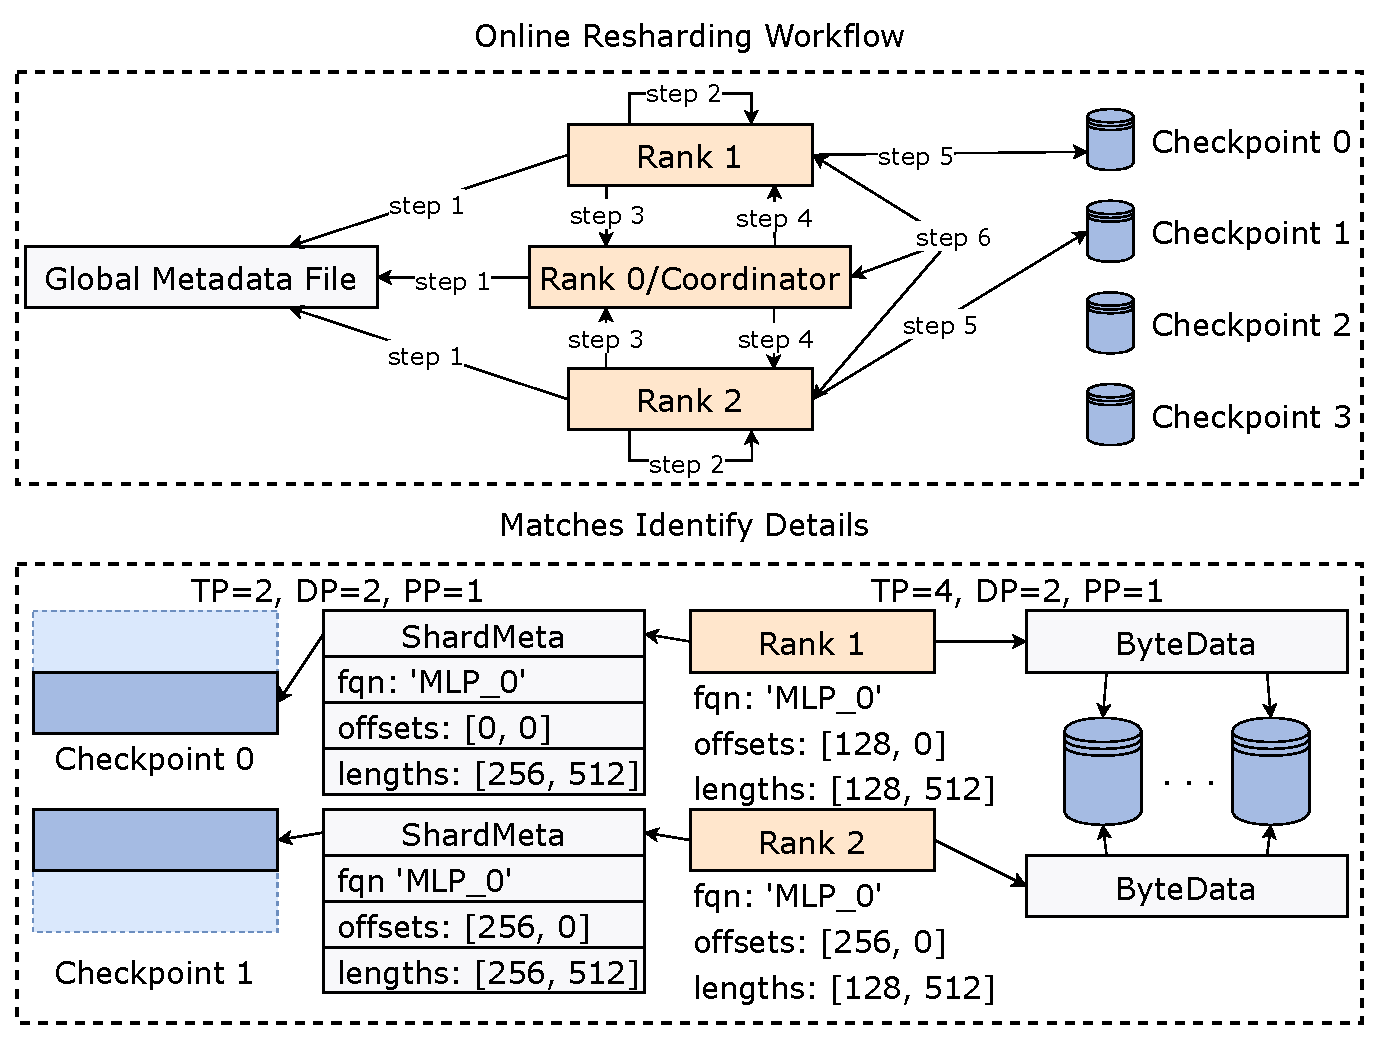
\includegraphics[width=\linewidth]{figures/tensor_reshard_examples.pdf}
  \caption{
  Load-time tensor resharding 工作流。
  Checkpoint $k$ 表示由先前运行的 worker $k$ 保存的 checkpoint。
  }
  \vspace{-5mm}
  \label{fig:tensor_reshard_example}
\end{figure}

\sys{} 实现了统一的保存/加载工作流，并在加载过程中自动 resharding。
借助 Engine、Planner 与 Storage I/O 层之间的解耦，我们可在不同训练框架与 storage backend 上执行一致的保存/加载步骤。
以下以 tensor resharding 为例（图~\ref{fig:tensor_reshard_example}），说明我们的 checkpoint 表示如何支持灵活的 load-time resharding。
对于不涉及 resharding 的保存与加载，流程类似。

\noindent \textbf{Step 1}。
每个 rank 调用 \texttt{bytecheckpoint.load()}，指定 checkpoint 路径以及待恢复的模型/优化器等状态。
所有 rank 从路径加载全局 metadata 文件。

\noindent \textbf{Step 2}。
对于模型/优化器中的每个 tensor shard，每个 rank 查询全局 metadata 中的 TensorShardToBasicByteMap，识别已保存 shards 与新分片规范之间的匹配片段。
识别完成后，planner 构建本地加载 plan，其中包含该 shard 对应的 BasicMeta 与 ByteMeta。
图~\ref{fig:tensor_reshard_example} 底部示意了这一匹配机制。

\noindent \textbf{Step 3}。
协调者 planner（通常位于 rank 0）发起 gather 操作汇总各 rank 的加载 plan，并应用冗余消除优化（Sec.~\ref{sec:opt_plan}）以分配加载工作量、缩短完成时间。

\noindent \textbf{Step 4}。
协调者发起 scatter 操作下发最终加载 plan，各 rank 接收其最终 plan。

\noindent \textbf{Step 5}。
每个 rank 的执行引擎根据 checkpoint 路径选择 Storage I/O 层中的 backend wrapper，并执行加载 pipeline（Sec.~\ref{sec:opt_pipeline}）。

\noindent \textbf{Step 6}。
加载 pipeline 完成后，各 rank 使用优化后的异步 collective barrier 原语确保分布式加载的原子性。
更多细节见附录~\ref{sec:barrier_check}。

\noindent \textbf{Dataloader resharding}。
类似图~\ref{fig:tensor_reshard_example} 的 tensor resharding，\sys{} 通过查询 LoaderShardtoByteMap 实现 dataloader resharding。
图~\ref{fig:loader_reshard_example} 展示了 dataloader resharding 的示意。
当 parallelism 配置变化时，dataloader checkpoints 中的公共条目可直接加载，而 token buffer 与数据读取偏移等独有条目需要 resharding。
具体而言，当 DP 度保持不变而其他 parallelism 度改变（图~\ref{fig:loader_reshard_example} 中 TP 改变）时，需要将 token buffer 复制到目标 worker 以保证 bitwise 正确的恢复；当 DP 度变化时，token buffer 需要相应拆分或合并，以确保恢复后的 dataloader 不会丢失缓存数据、也不会重复训练已采样的数据。
得益于 dataloader 模块的分拆存储策略，\sys{} 能精确识别需要 resharding 的独有条目并高效处理。

\begin{figure}[!t]
  \centering
  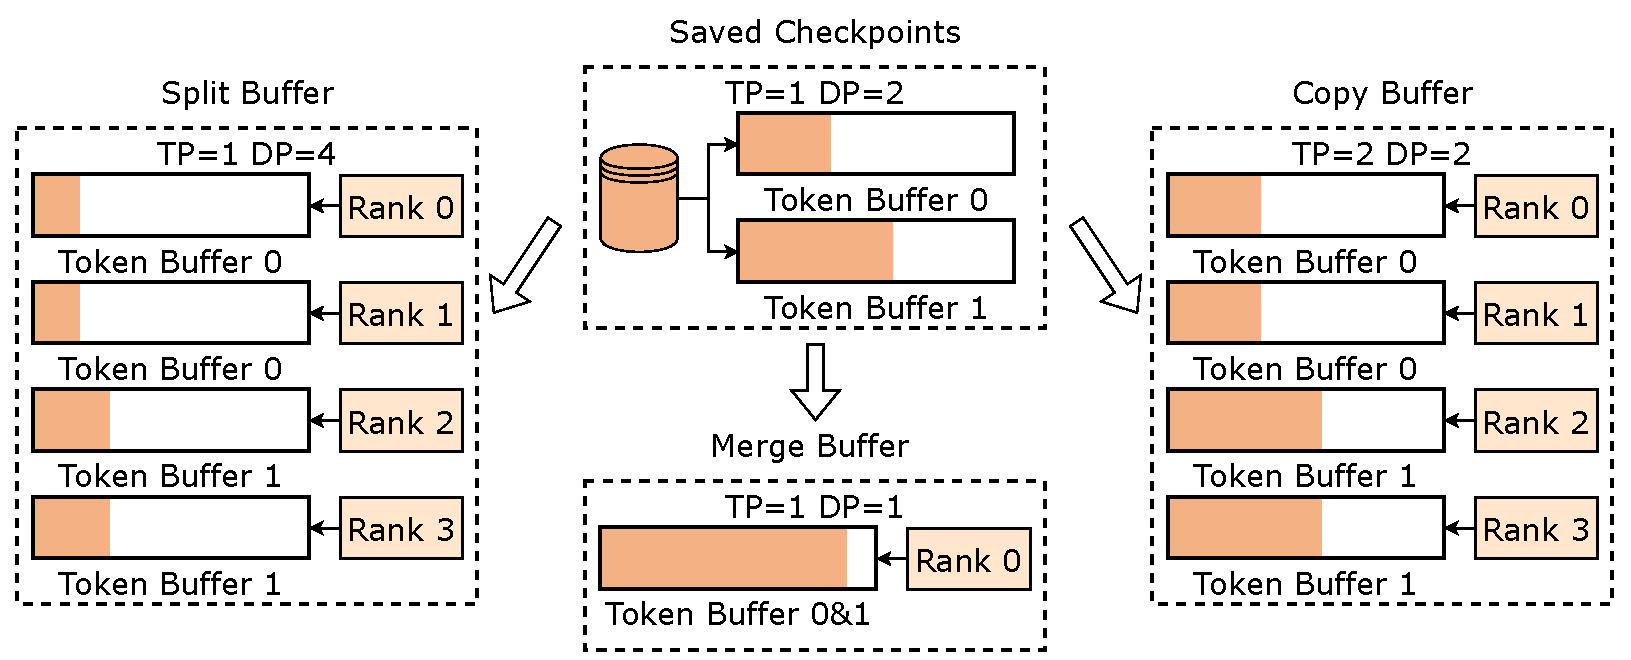
\includegraphics[width=\linewidth]{figures/loader_reshard_examples.pdf}
  \caption{
  Dataloader resharding 示例。
  并行配置变化时，对 cumulative token buffer 等 sharded 状态进行 resharding。
  为清晰起见，图中未绘制数据读取偏移。
  }
  \label{fig:loader_reshard_example}
\end{figure}

